%% LyX 2.4.4 created this file.  For more info, see https://www.lyx.org/.
%% Do not edit unless you really know what you are doing.
\documentclass[english]{article}
\usepackage[T1]{fontenc}
\usepackage[latin9]{inputenc}
\usepackage{enumitem}
\usepackage{amsmath}
\usepackage{amsthm}
\usepackage{cancel}
\usepackage{geometry}
\geometry{verbose,tmargin=1in,bmargin=1in,lmargin=1in,rmargin=1in}

\makeatletter

%%%%%%%%%%%%%%%%%%%%%%%%%%%%%% LyX specific LaTeX commands.
%% Because html converters don't know tabularnewline
\providecommand{\tabularnewline}{\\}

%%%%%%%%%%%%%%%%%%%%%%%%%%%%%% Textclass specific LaTeX commands.
\numberwithin{equation}{section}
\numberwithin{figure}{section}
\newlength{\lyxlabelwidth}      % auxiliary length 

%%%%%%%%%%%%%%%%%%%%%%%%%%%%%% User specified LaTeX commands.
\usepackage{hyperref}
\usepackage[usenames,dvipsnames,table]{xcolor} %adds additional color options
\hypersetup{colorlinks=true, urlcolor=black}

\usepackage{fancyhdr}
\usepackage{lastpage}
\pagestyle{fancy}
\usepackage{enumitem}
\usepackage{ifthen}
%sets math fonts to be more readable
\everymath=\expandafter{\the\everymath\displaystyle}
%\DeclareMathSizes{10}{10}{10}{10}
\usepackage{multicol}

\usepackage{tikz}
\usetikzlibrary{plotmarks}
\usepackage{pgfplots}
\pgfplotsset{compat=newest}

\usepackage{calc}
\usepackage[nomessages]{fp}

\usepackage{advdate}    % Advancing/saving dates
\usepackage{datetime}   % Dates formatting
\usepackage{datenumber} % Counters for dates

\usepackage{fancybox} %%ovalbox and fancy box settings

\usepackage[outline]{contour}  %allows text halos
\usepackage{colortbl}
% Added by lyx2lyx
\setlength{\parskip}{\smallskipamount}
\setlength{\parindent}{0pt}

\makeatother

\usepackage{babel}
\begin{document}
\renewcommand{\author}{Dr.\,James Ashe}

\newcommand{\classNum}{107}

\newcommand{\classSec}{7 and 10}

\newcommand{\nameType}{}

\newcommand{\examType}{Exam 2 Review: sections 1.1-1.5}

\renewcommand{\date}{\hfill Exam 2 is on \formatdate{1}{10}{2014}}

%%First page's header%%%%%%%%%%%%%%%%%%%%%%
\fancypagestyle{firststyle} %%header settings for first pagr
{
	\fancyhead[L]{MTH \classNum{}(\classSec{}) \author{}\\
	\textbf{\examType{}} \date{}}
	\fancyhead[C]{\textbf{\nameType}}
	\setlength{\headsep}{14pt}
}
%%%%%%%%%%%%%%%%%%%%%%%%%%%%%%%%%%%%%%%%%%

%%Next page's header%%%%%%%%%%%%%%%%%%%%%%%
%\setlist{nolistsep}
\lhead{MTH \classNum{}(\classSec{})} 
\chead{\textbf{\nameType}} 
\cfoot{\thepage{}~of~\pageref{LastPage}} 
\setlength{\headsep}{5pt} 
%%%%%%%%%%%%%%%%%%%%%%%%%%%%%%%%%%%%%%%%%%%

%%Various settings; see the preamble for other settings%%%%%
%%\setenumerate[0]{leftmargin=12pt,itemindent=0pt,labelwidth=0pt}
%\setlist[2]{noitemsep}
%\setlist{nosep}
\setlist{itemsep=-3pt,topsep=-2pt}
\renewcommand{\labelenumi}{\textbf{\arabic{enumi}.}}
\renewcommand{\labelenumii}{\textbf{\alph{enumii}.}}
\thispagestyle{firststyle}
%%%%%%%%%%%%%%%%%%%%%%%%%%%%%%%%%%%%%%%%%%
\newcommand{\xmax}{10}
\newcommand{\xmin}{-10}
\newcommand{\xstep}{0} %must be xmin+n
\newcommand{\ymax}{10}
\newcommand{\ymin}{-10}
\newcommand{\ystep}{0} %must be ymin+n

\newcommand{\xspace}{\hspace*{40pt}}
\newcommand{\yspace}{\vspace*{.25cm}}
\newcommand{\rowColor}{gray!35}
\begin{enumerate}[resume]
\item Construct a Venn diagram to determine the validity of the given argument.

\begin{enumerate}
\item \vspace{-25pt} \begin{multicols}{2}%
\begin{tabular}{l}
\tabularnewline
\tabularnewline
1. All basketball players are well conditioned.\tabularnewline
2. Bill is well-conditioned.\tabularnewline
\hline 
Therefore, Bill is a basketball player. \tabularnewline
\textbf{Invalid}\tabularnewline
\end{tabular}\columnbreak\\
\vfill \hfill%%%%little circle in big%%%%%
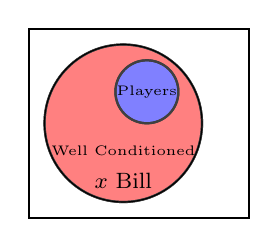
\begin{tikzpicture}[scale=.4]
	\def\circleA{(1,-1) circle (2.5)} %A
	\def\circleB{(0:1.75) circle (1)} %B

	\colorlet{circle edgeA}{black!75} 
	\colorlet{circle areaA}{red!50}
	\colorlet{circle edgeB}{black!75} 
	\colorlet{circle areaB}{blue!50}

	\tikzset{
		filledA/.style={fill=circle areaA, draw=circle edgeA, thick},
		filledB/.style={fill=circle areaB, draw=circle edgeB, thick},
		outlineA/.style={draw=circle edgeA, thick},
		outlineB/.style={draw=circle edgeB, thick},
	}

	\begin{scope}[fill opacity=1.0]         
			\fill[filledA] \circleA;
			\fill[filledB] \circleB;    
	\end{scope}
	
	\footnotesize
	\draw[outlineA] \circleA node[below = 5pt] {\tiny Well Conditioned} node[below = 10pt] {$$}; 
	\draw[outlineB] \circleB node {\tiny Players} node[below = 5pt] {$$};
	%\node[anchor=south] at (current bounding box.north) {$A \cup B$}; 
	\draw[thick] (-2,-4) rectangle (5,2) node[anchor=south east] at (current bounding box.south east) {};
	\draw \circleA node[below=15pt] {\footnotesize $x$ Bill};
\end{tikzpicture} \hspace{2cm}

\end{multicols}\yspace
\item \vspace{-25pt} \begin{multicols}{2}%
\begin{tabular}{l}
\tabularnewline
\tabularnewline
1. All pilots must take a drug test.\tabularnewline
2. Some people who take drug tests get false positives.\tabularnewline
\hline 
Therefore, some pilots get false-positives. \tabularnewline
\textbf{Invalid}\tabularnewline
\end{tabular}\columnbreak\\
\vfill \hfill%%%%little circle in big%%%%%
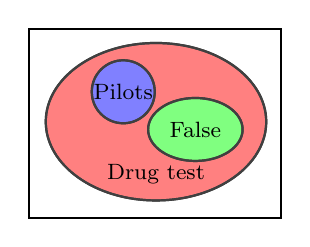
\begin{tikzpicture}[scale=.4]
	\def\circleA{(-25:2.25) ellipse (3.5 and 2.5)} %A
	\def\circleB{(0:1) circle (1)} %B
	\def\circleC{(-20:3.5) ellipse (1.5 and 1)} %C


	\colorlet{circle edgeA}{black!75} 
	\colorlet{circle areaA}{red!50}
	\colorlet{circle edgeB}{black!75} 
	\colorlet{circle areaB}{blue!50}
	\colorlet{circle edgeC}{black!75} 
	\colorlet{circle areaC}{green!50}

	\tikzset{
		filledA/.style={fill=circle areaA, draw=circle edgeA, thick},
		filledB/.style={fill=circle areaB, draw=circle edgeB, thick},
		filledC/.style={fill=circle areaC, draw=circle edgeC, thick},
		outlineA/.style={draw=circle edgeA, thick},
		outlineB/.style={draw=circle edgeB, thick},
		outlineC/.style={draw=circle edgeC, thick}
	}

	\begin{scope}[fill opacity=1.0]         
			\fill[filledA] \circleA;
			\fill[filledB] \circleB;
			\fill[filledC] \circleC;  
	\end{scope}
	
	\footnotesize
	\draw[outlineA] \circleA node[below = 12pt] {Drug test} node[below = 15pt] {$$}; 
	\draw[outlineB] \circleB node {Pilots} node[below = 5pt] {$$};
	\draw[outlineC] \circleC node {False} node[below = 5pt] {$$};
	%\node[anchor=south] at (current bounding box.north) {$A \cup B$}; 
	\draw[thick] (-2,-4) rectangle (6,2) node[anchor=south east] at (current bounding box.south east) {$$};
	%\draw \circleA node[below=30pt,right=0pt] {\footnotesize{\emph{Gates}}};
\end{tikzpicture} \hspace{2cm}

\end{multicols}\yspace
\item \vspace{-25pt} \begin{multicols}{2}%
\begin{tabular}{l}
\tabularnewline
\tabularnewline
1. All squares are rectangles.\tabularnewline
2. Some quadrilaterals are squares.\tabularnewline
\hline 
Therefore, some quadrilaterals are rectangles. \tabularnewline
\textbf{Valid}\tabularnewline
\end{tabular}\columnbreak\\
\vfill \hfill%%%%little circle in big%%%%%
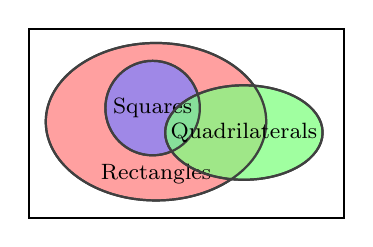
\begin{tikzpicture}[scale=.4]
	\def\circleA{(-25:2.25) ellipse (3.5 and 2.5)} %A
	\def\circleB{(-15:2) circle (1.5)} %B
	\def\circleC{(-15:5) ellipse (2.5 and 1.5)} %C


	\colorlet{circle edgeA}{black!75} 
	\colorlet{circle areaA}{red!50}
	\colorlet{circle edgeB}{black!75} 
	\colorlet{circle areaB}{blue!50}
	\colorlet{circle edgeC}{black!75} 
	\colorlet{circle areaC}{green!50}

	\tikzset{
		filledA/.style={fill=circle areaA, draw=circle edgeA, thick},
		filledB/.style={fill=circle areaB, draw=circle edgeB, thick},
		filledC/.style={fill=circle areaC, draw=circle edgeC, thick},
		outlineA/.style={draw=circle edgeA, thick},
		outlineB/.style={draw=circle edgeB, thick},
		outlineC/.style={draw=circle edgeC, thick}
	}

	\begin{scope}[fill opacity=.75]         
			\fill[filledA] \circleA;
			\fill[filledB] \circleB;
			\fill[filledC] \circleC;  
	\end{scope}
	
	\footnotesize
	\draw[outlineA] \circleA node[below = 12pt] {Rectangles} node[below = 15pt] {$$}; 
	\draw[outlineB] \circleB node {Squares} node[below = 5pt] {$$};
	\draw[outlineC] \circleC node {Quadrilaterals} node[below = 5pt] {$$};
	%\node[anchor=south] at (current bounding box.north) {$A \cup B$}; 
	\draw[thick] (-2,-4) rectangle (8,2) node[anchor=south east] at (current bounding box.south east) {$$};
	%\draw \circleA node[below=30pt,right=0pt] {\footnotesize{\emph{Gates}}};
\end{tikzpicture} \hspace{2cm}

\end{multicols}\yspace
\end{enumerate}
\item Using the symbolic representations\\
\begin{tabular}{rl}
$b$: & I ride a bicycle to school.\tabularnewline
$s$: & It is snowing.\tabularnewline
$r$: & It is raining. \tabularnewline
\end{tabular}\\
express the following statements in symbolic form.

\begin{enumerate}
\item It is raining and I rode my bicycle to school.

\begin{enumerate}
\item []$r\wedge b$\yspace
\end{enumerate}
\item If it is raining or snowing, then I will not ride my bicycle to school.

\begin{enumerate}
\item []$(r\vee s)\rightarrow\sim b$\yspace
\end{enumerate}
\end{enumerate}
\item Let $x$ be an integer. Using the symbolic representations\\
\begin{tabular}{rl}
$p$: & $x$ is a prime number.\tabularnewline
$o$: & $x$ is odd.\tabularnewline
$t$: & $x$ is equal to $2$.\tabularnewline
$e$: & $x$ is divisible by $8$.\tabularnewline
\end{tabular}\\
express the following in words.

\begin{enumerate}
\item $p\rightarrow(o\vee t)$

\begin{enumerate}
\item []If $\underset{p}{\underbrace{\mbox{\emph{x }is a prime number}}}$
then $\underset{o}{\underbrace{\mbox{\emph{x }is odd}}}$ or $\underset{t}{\underbrace{\mbox{\emph{x }is equal to 2}}}$.\yspace
\end{enumerate}
\item $e\rightarrow\sim p$

\begin{enumerate}
\item []If $\underset{t}{\underbrace{\mbox{\emph{x }is divisible by 8}}}$
then $\underset{\sim p}{\underbrace{\mbox{\emph{x }is not prime}}}$.\yspace
\end{enumerate}
\item $\sim o\vee\sim e$

\begin{enumerate}
\item []If $\underset{\sim o}{\underbrace{\mbox{\emph{x }is not odd}}}$
or $\underset{\sim e}{\underbrace{\mbox{\emph{x }is not even}}}$.\yspace
\end{enumerate}
\item $\sim(o\wedge e)\wedge t$

\begin{enumerate}
\item []It is not the case that $\underset{o}{\underbrace{\mbox{\emph{x }is odd}}}$
and $\underset{e}{\underbrace{\mbox{\emph{x }is even}}}$, and $\underset{e}{\underbrace{\mbox{\emph{x }is equal to 2}}}$.\yspace\newpage
\end{enumerate}
\end{enumerate}
\item Construct a truth table for the symbolic expression.\newcommand{\T}{\textcolor{green}{\contour{black}{T}}}
\newcommand{\F}{\textcolor{red}{\contour{black}{F}}}\begin{multicols}{2}

\begin{enumerate}
\item $p\wedge(q\rightarrow\sim p)$\\
\begin{tabular}{c|c|c|c|c}
$p$ & $q$ & $\sim p$ & $q\rightarrow\sim p$ & $p\wedge(q\rightarrow\sim p)$\tabularnewline
\hline 
\hline 
\rowcolor{gray!50}T & T & \F & \F & \F\tabularnewline
\hline 
T & F & \F & \T & \T\tabularnewline
\hline 
\rowcolor{gray!50}F & T & \T & \T & \F\tabularnewline
\hline 
F & F & \T & \T & \F\tabularnewline
\multicolumn{1}{c}{} & \multicolumn{1}{c}{} & \multicolumn{1}{c}{\xspace } & \multicolumn{1}{c}{\xspace} & \xspace\tabularnewline
\end{tabular}\yspace
\item $(x\rightarrow y)\vee\sim x$\\
\begin{tabular}{c|c|c|c|c}
$x$ & $y$ & $x\rightarrow y$ & $\sim x$ & $(x\rightarrow y)\vee x$\tabularnewline
\hline 
\hline 
\rowcolor{gray!50}T & T & \T & \F & \T\tabularnewline
\hline 
T & F & \F & \F & \T\tabularnewline
\hline 
\rowcolor{gray!50}F & T & \T & \T & \T\tabularnewline
\hline 
F & F & \T & \T & \T\tabularnewline
\multicolumn{1}{c}{} & \multicolumn{1}{c}{} & \multicolumn{1}{c}{\xspace } & \multicolumn{1}{c}{\xspace} & \xspace\tabularnewline
\end{tabular}\yspace
\end{enumerate}
\end{multicols}
\begin{enumerate}[resume]
\item [\textbf{c.}]$\sim a\wedge(b\rightarrow c)$\\
\begin{tabular}{c|c|c|c|c|c}
$a$ & $b$ & \textbf{$c$} & $\sim a$ & $b\rightarrow c$ & $\sim a\wedge(b\rightarrow c)$\tabularnewline
\hline 
\hline 
\rowcolor{gray!50}T & T & T & \F & \T & \F\tabularnewline
\hline 
T & T & F & \F & \F & \F\tabularnewline
\hline 
\rowcolor{gray!50}T & F & T & \F & \T & \F\tabularnewline
\hline 
T & F & F & \F & \T & \F\tabularnewline
\hline 
\rowcolor{gray!50}F & T & T & \T & \T & \T\tabularnewline
\hline 
F & T & F & \T & \F & \F\tabularnewline
\hline 
\rowcolor{gray!50}F & F & T & \T & \T & \T\tabularnewline
\hline 
F & F & F & \T & \T & \T\tabularnewline
\multicolumn{1}{c}{} & \multicolumn{1}{c}{} & \multicolumn{1}{c}{} & \multicolumn{1}{c}{\xspace } & \multicolumn{1}{c}{\xspace} & \xspace\tabularnewline
\end{tabular}\yspace
\end{enumerate}
\item Symbolically write the negation of the following statements.

\begin{enumerate}
\item The grass is not greener.

\begin{enumerate}
\item []%
\begin{tabular}{ll}
$g$: & The grass is greener.\tabularnewline
\end{tabular}\\
Statement: $g$\\
Negation: $\sim g$\yspace
\end{enumerate}
\item It is not the case that, if our car is not fixed then we cannot drive
to Asheville. 

\begin{enumerate}
\item []%
\begin{tabular}{rl}
$f$: & Our car is fixed.\tabularnewline
$d$: & We can drive to Asheville.\tabularnewline
\end{tabular}\\
Statement: $\sim(\sim f\rightarrow\sim d)$\\
Negation: $\sim\left(\sim(f\rightarrow\sim d)\right)\equiv\sim f\rightarrow\sim d$\yspace
\end{enumerate}
\end{enumerate}
\item Write the negation of the following statements.

\begin{enumerate}
\item Some freshmen are taking Math 107.

\begin{enumerate}
\item []\emph{No }freshmen are taking Math 107.\yspace
\end{enumerate}
\item Some seniors are not taking Math 107.

\begin{enumerate}
\item [] \emph{All }seniors are taking Math 107. \yspace
\end{enumerate}
\item All football players need to attend practice.

\begin{enumerate}
\item []\emph{Some} football players \emph{do not} need to attend practice.\yspace
\end{enumerate}
\item No professors attend football practice.

\begin{enumerate}
\item []\emph{Some }professors do attend football practice.\yspace
\end{enumerate}
\end{enumerate}
\item Using the statement, ``If your order is over \$50, then you will
not have to pay shipping fees.'' write the following:\emph{}\\
\begin{tabular}{rlrl}
$o$: & The order is over \$50. &  & \tabularnewline
$p$: & You have to pay shipping fees. & Statement: & $o\rightarrow\sim p$\tabularnewline
\end{tabular}

\begin{enumerate}
\item \textbf{Converse}:

\begin{enumerate}
\item [$\sim p\rightarrow o$:]If $\underset{\sim p}{\underbrace{\mbox{you do not have to pay shipping fees}}}$
then $\underset{o}{\underbrace{\mbox{your order is over \$50}}}$.\yspace
\end{enumerate}
\item \textbf{Inverse}:

\begin{enumerate}
\item [$\sim o\rightarrow\sim(\sim p)$:]If $\underset{\sim o}{\underbrace{\mbox{your order is not over \$50}}}$
then $\underset{\sim(\sim p)\equiv p}{\underbrace{\mbox{you have to pay shipping fees}}}$.\yspace
\end{enumerate}
\item \textbf{Contrapositive:}

\begin{enumerate}
\item [$\sim(\sim p)\rightarrow\sim o$:]If $\underset{\sim(\sim p)\equiv p}{\underbrace{\mbox{you have to pay shipping fees}}}$
then $\underset{\sim o}{\underbrace{\mbox{your order is not over \$50}}}$.\yspace
\end{enumerate}
\item \textbf{Contrapositive }in terms of a sufficient condition\textbf{:}

\begin{enumerate}
\item [$\sim(\sim p)\rightarrow\sim o$:]$\underset{\sim(\sim p)\equiv p}{\underbrace{\mbox{Having to pay shipping fees}}}$
is sufficient for $\underset{\sim o}{\underbrace{\mbox{your order to be not over \$50}}}$.\yspace
\end{enumerate}
\item \textbf{Negation }using conjunction\textbf{:}

\begin{enumerate}
\item [$\sim(o\rightarrow\sim p)$:] Using De Morgan's law, $\sim(o\rightarrow\sim p)\equiv o\wedge\sim(\sim p)\equiv o\wedge p$\\
$\underset{o}{\underbrace{\mbox{Your order is over \$50}}}$ and $\underset{p}{\underbrace{\mbox{you have to pay shipping fees}}}$.\yspace
\end{enumerate}
\end{enumerate}
\item Using the statement, ``If the sun is going down, then the cows are
coming home.'' write the following:\\
\begin{tabular}{rlrl}
$s$: & The sun is going down. &  & \tabularnewline
$c$: & The cows are coming home. & Statement: & $s\rightarrow c$\tabularnewline
\end{tabular}

\begin{enumerate}
\item \textbf{Converse}:

\begin{enumerate}
\item [$c\rightarrow s$:]If $\underset{c}{\underbrace{\mbox{the cows are coming home}}}$
then $\underset{s}{\underbrace{\mbox{the sun is going down}}}$.\yspace
\end{enumerate}
\item \textbf{Inverse}:

\begin{enumerate}
\item [$\sim s\rightarrow\sim c$:]If $\underset{\sim s}{\underbrace{\mbox{the sun is not going down}}}$
then $\underset{\sim c}{\underbrace{\mbox{the cows are not coming home}}}$.\yspace
\end{enumerate}
\item \textbf{Contrapositive:}

\begin{enumerate}
\item [$\sim c\rightarrow\sim s$:]If $\underset{\sim c}{\underbrace{\mbox{the cows are not coming home}}}$
then $\underset{\sim s}{\underbrace{\mbox{the sun is not going down}}}$.\yspace
\end{enumerate}
\item \textbf{Contrapositive }in terms of a necessary condition\textbf{:}

\begin{enumerate}
\item [$\sim c\rightarrow\sim s$:]$\underset{\sim s}{\underbrace{\mbox{The sun not going down}}}$
is necessary $\underset{\sim c}{\underbrace{\mbox{for the cows not coming home}}}$.\yspace
\end{enumerate}
\item \textbf{Negation }using conjunction\textbf{:}

\begin{enumerate}
\item [$\sim(c\rightarrow s)$:] Using De Morgan's law, $\sim(c\rightarrow s)\equiv c\wedge\sim s$\\
$\underset{\sim c}{\underbrace{\mbox{The cows are coming home}}}$
and $\underset{\sim s}{\underbrace{\mbox{the sun is not going down}}}$.\yspace
\end{enumerate}
\end{enumerate}
\item Use a truth table to determine if the following arguments are valid.

\begin{enumerate}
\item \vspace{-25pt}%
\begin{tabular}{rll}
 &  & \tabularnewline
 &  & \tabularnewline
$b$: & You buy the bike. & 1. You buy the bike or the tent.\tabularnewline
$t$: & You buy the tent. & 2. You buy the bike.\tabularnewline
\cline{3-3}
 &  & Therefore, you do not buy the tent.\tabularnewline
\end{tabular}\\
\begin{tabular}{c|c|c|c|c|c|c}
\multicolumn{1}{c}{} & \multicolumn{1}{c}{} & \multicolumn{1}{c}{\xspace} & \multicolumn{1}{c}{\xspace} & \multicolumn{1}{c}{\xspace} & \multicolumn{1}{c}{\xspace} & \xspace\tabularnewline
\multicolumn{1}{c}{} & \multicolumn{1}{c}{} & \multicolumn{1}{c}{\ovalbox{$1$}} & \multicolumn{1}{c}{\ovalbox{$2$}} & \multicolumn{1}{c}{} & \multicolumn{1}{c}{\ovalbox{$c$}} & \ovalbox{Argument}\tabularnewline
$b$ & $t$ & $b\vee t$ & $b$ & $1 \wedge 2$ & $\sim t$ & $\left(1\wedge2\right)\rightarrow c$\tabularnewline
\hline 
\hline 
\rowcolor{\rowColor}T & T & \T & \T & \T & \F & \fbox{\F}\tabularnewline
\hline 
T & F & \T & \T & \T & \T & \T\tabularnewline
\hline 
\rowcolor{\rowColor}F & T & \T & \F & \F & \F & \T\tabularnewline
\hline 
F & F & \F & \F & \F & \T & \T\tabularnewline
\end{tabular}

\begin{enumerate}
\item []The argument is not always true so it is,\textbf{ invalid}\yspace
\end{enumerate}
\item \vspace{-25pt} %
\begin{tabular}{rll}
 &  & \tabularnewline
 &  & \tabularnewline
$r$: & You register early. & 1. If you register early, then you will receive a discount.\tabularnewline
$d$: & You receive a discount. & 2. You register early.\tabularnewline
\cline{3-3}
 &  & Therefore, you will receive a discount.\tabularnewline
\end{tabular}\\
\begin{tabular}{c|c|c|c|c|c|c}
\multicolumn{1}{c}{} & \multicolumn{1}{c}{} & \multicolumn{1}{c}{\xspace} & \multicolumn{1}{c}{\xspace} & \multicolumn{1}{c}{\xspace} & \multicolumn{1}{c}{\xspace} & \xspace\tabularnewline
\multicolumn{1}{c}{} & \multicolumn{1}{c}{} & \multicolumn{1}{c}{\ovalbox{$1$}} & \multicolumn{1}{c}{\ovalbox{$2$}} & \multicolumn{1}{c}{} & \multicolumn{1}{c}{\ovalbox{$c$}} & \ovalbox{Argument}\tabularnewline
$r$ & $d$ & $r\rightarrow d$ & $r$ & $1 \wedge 2$ & $r$ & $\left(1\wedge2\right)\rightarrow c$\tabularnewline
\hline 
\hline 
\rowcolor{\rowColor}T & T & \T & \T & \T & \T & \T\tabularnewline
\hline 
T & F & \F & \T & \F & \T & \T\tabularnewline
\hline 
\rowcolor{\rowColor}F & T & \T & \F & \F & \F & \T\tabularnewline
\hline 
F & F & \T & \F & \F & \F & \T\tabularnewline
\end{tabular}

\begin{enumerate}
\item []The argument is always true so it is, \textbf{valid}\yspace
\end{enumerate}
\item \vspace{-25pt}%
\begin{tabular}{rll}
 &  & \tabularnewline
 &  & \tabularnewline
$b$: & You buy the property. & 1. If you buy the property, then you will need a loan.\tabularnewline
$n$: & You need a loan. & 2. If you need a loan, then you will pay 8\%.\tabularnewline
\cline{3-3}
$p$: & You will pay 8\%. & Therefore, if you buy the property then you will pay 8\%.\tabularnewline
\end{tabular}\\
\begin{tabular}{c|c|c|c|c|c|c|c}
\multicolumn{1}{c}{} & \multicolumn{1}{c}{} & \multicolumn{1}{c}{} & \multicolumn{1}{c}{\xspace} & \multicolumn{1}{c}{\xspace} & \multicolumn{1}{c}{\xspace} & \multicolumn{1}{c}{\xspace} & \xspace\tabularnewline
\multicolumn{1}{c}{} & \multicolumn{1}{c}{} & \multicolumn{1}{c}{} & \multicolumn{1}{c}{\ovalbox{$1$}} & \multicolumn{1}{c}{\ovalbox{$2$}} & \multicolumn{1}{c}{} & \multicolumn{1}{c}{\ovalbox{$c$}} & \ovalbox{Argument}\tabularnewline
$b$ & $n$ & $p$ & $b\rightarrow n$ & $n\rightarrow p$ & $1\wedge2$ & $b\rightarrow p$ & $(1\wedge2)\rightarrow c$\tabularnewline
\hline 
\hline 
\rowcolor{\rowColor}T & T & T & \T & \T & \T & \T & \T\tabularnewline
\hline 
T & T & F & \T & \F & \F & \F & \T\tabularnewline
\hline 
\rowcolor{\rowColor}T & F & T & \F & \T & \F & \T & \T\tabularnewline
\hline 
T & F & F & \F & \T & \F & \F & \T\tabularnewline
\hline 
\rowcolor{\rowColor}F & T & T & \T & \T & \T & \T & \T\tabularnewline
\hline 
F & T & F & \T & \F & \F & \T & \T\tabularnewline
\hline 
\rowcolor{\rowColor}F & F & T & \T & \T & \T & \T & \T\tabularnewline
\hline 
F & F & F & \T & \T & \T & \T & \T\tabularnewline
\end{tabular}

\begin{enumerate}
\item []The argument is always true so it is, \textbf{valid}\yspace
\end{enumerate}
\item \vspace{-25pt}%
\begin{tabular}{lrl}
 &  & \tabularnewline
 &  & \tabularnewline
1. Nothing intelligible ever puzzles me. & $i$: & It is intelligible.\tabularnewline
2. Logic puzzles me. & $p$: & It puzzles me.\tabularnewline
\cline{1-1}
Therefore, logic is unintelligible.  & $\ell$: & It is logic.\tabularnewline
\end{tabular}\\
\begin{tabular}{c|c|c|c|c|c|c|c|c|c}
\multicolumn{1}{c}{} & \multicolumn{1}{c}{} & \multicolumn{1}{c}{} & \multicolumn{1}{c}{\xspace} & \multicolumn{1}{c}{\xspace} & \multicolumn{1}{c}{\xspace} & \multicolumn{1}{c}{\xspace} & \multicolumn{1}{c}{\xspace} & \multicolumn{1}{c}{\xspace} & \xspace\tabularnewline
\multicolumn{1}{c}{} & \multicolumn{1}{c}{} & \multicolumn{1}{c}{} & \multicolumn{1}{c}{} & \multicolumn{1}{c}{\Ovalbox{1}} & \multicolumn{1}{c}{\Ovalbox{2}} & \multicolumn{1}{c}{} & \multicolumn{1}{c}{} & \multicolumn{1}{c}{\Ovalbox{c}} & \ovalbox{Argument}\tabularnewline
$i$ & $p$ & $\ell$ & $\sim p$ & $i\rightarrow\sim p$ & $\ell\rightarrow p$ & $1\wedge2$ & $\sim i$ & $\ell\rightarrow\sim i$ & $(1\wedge2)\rightarrow c$\tabularnewline
\hline 
\hline 
\rowcolor{\rowColor}T & T & T & \F & \F & \T & \F & \F & \F & \T\tabularnewline
\hline 
T & T & F & \F & \F & \T & \F & \F & \T & \T\tabularnewline
\hline 
\rowcolor{\rowColor}T & F & T & \T & \T & \F & \F & \F & \F & \T\tabularnewline
\hline 
T & F & F & \T & \T & \T & \T & \F & \T & \T\tabularnewline
\hline 
\rowcolor{\rowColor}F & T & T & \F & \T & \T & \T & \T & \T & \T\tabularnewline
\hline 
F & T & F & \F & \T & \T & \T & \T & \T & \T\tabularnewline
\hline 
\rowcolor{\rowColor}F & F & T & \T & \T & \F & \F & \T & \T & \T\tabularnewline
\hline 
F & F & F & \T & \T & \T & \T & \T & \T & \T\tabularnewline
\end{tabular}

\begin{enumerate}
\item []The argument is always true so it is, \textbf{valid}\yspace
\end{enumerate}
\end{enumerate}
\end{enumerate}

\end{document}
